\section{Chapter 5: Visual salience and finding information}
\graphicspath{ {pngs/ch5/} }
%    \begin{figure}[H]
%        \centering
%        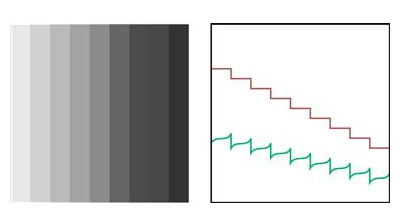
\includegraphics[width=0.4\textwidth]{chevreul_illusion.png}
%        \caption{Chevreul illusion, grayscale step patterns}
%    \end{figure}


\secttoc

\textbf{Symbol} is an object representing an entity.
\textbf{Glyph} is a symbol meant to convey one or more numerical attributes
of that entity.
We mostly see what we expect to see.
Glyphs must stand out in at least one channel.
For low-level properties, like interferes with like.
Channels can be separable or holistic.
Must make fundamental design choices and tradeoffs.

\begin{mdframed}\begin{multicols}{2}
\subsection{Eye movements}
\begin{compactdesc}
    \item[Saccades] a fast change of focus. 2-5 per second while reading.
        Said to be \emph{ballistic}, they cannot be adjusted mid-movement.
    \item[Saccadic suppression] During such a movement, we are less sensitive
        to visual input.
    \item[Saccadic movements] Rapid movement between fixations.
        Dwell period between 200 and 400 msec.
        Saccade takes 20 to 180 msec, depends on angle. 2 degrees while
        reading. 2 to 5 degrees is good.
    \item[Smooth-pursuit movements] eye can pursue smooth moving objects. Can
        also make head/body movements to follow.
    \item[Convergent movements] Also called vergence movements. When an object moves
        towards us, eyes converge. Moves away, eyes diverge. Can be either
        saccadic or smooth.
    \item[Accomodation] refocusing takes about 200 msec. Ability declines with
        age, fix with different-lens glasses or laser surgery (one near, one
        far).
\end{compactdesc}

\subsubsection{What is easily findable?}
How do we know where to look next? Heuristics strategy: focus on features that
fit our goal most closely.
\begin{compactdesc}
    \item[A priori salience] some patterns excite more neural activity than
        others.
    \item[Top-down salience modification] Depends on our goal. We can focus on
        relevant low-level V1 features.
    \item[Scene gist] Less about feature maps, more experience. Eye movements
        can be primed to specific types of learned scenes.
\end{compactdesc}
\end{multicols}\end{mdframed}



\begin{mdframed}\begin{multicols}{2}
    \begin{figure}[H]
        \centering
        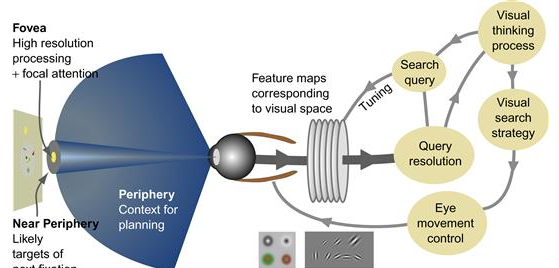
\includegraphics[width=\linewidth]{visual_search.png}
        \caption{The process of visual search}
    \end{figure}
    \begin{figure}[H]
        \centering
        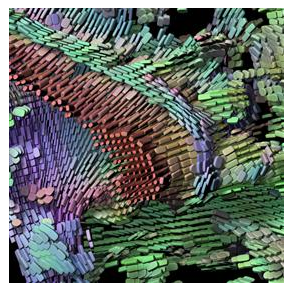
\includegraphics[width=0.6\linewidth]{tensor_vis.png}
        \caption{3D tensor field visualization using color, orientation and
        shape.}
    \end{figure}


\end{multicols}\end{mdframed}


\begin{mdframed}\begin{multicols}{2}
\subsection{V1, Channels, and Tuned Receptors}
\begin{compactdesc}
    \item[V1 and V2] V1 passes mostly to V2, they represent 40\% of vision
        processing. Several billion neurons devoted to analyzing output from
        several million nerve fibers.
    \item[Optic nerves] split the image into red-green, yellow-blue and
        dark-light channels before sending to V1.
    \item[Semi-independent features] processed by V1, V2:
        \begin{compactenum}
        \item Orientation and size (with luminance)
        \item Color via opponent processing
        \item Elements of local stereoscopic depth
        \item Elements of local motion
        \end{compactenum}
        A feature close to another feature is processed by nearby neurons.
    \item[Elements of form] These features are like phonemes in speech.
        Can be independent of each other. Color, form and motion.
        More complex composite patterns aren't processed as rapidly.
    \item[Assumption:] single neurons can be treated as independent.
        Groups of neurons or synchronization or temporal spacing also encode
        information, maybe more?
    \item[V1 and V2] continually process orientation and size. Each of the stages
        has a preferred size/orientation.
    \item[Gabor model and visual distinctness] Simple mathematical model:
        multiply a cosine wave by a Gaussian envelope. Excitory center flanked
        by two inhibitory bars. Variables: amplitude/contrast, size, and
        rotation. Detect particular orientations but not right-angles.
    \item[Barlow's 2nd dogma] fits with Gabor model. Simultaneously optimized
        for spatial location, size and orientation.
    \item[Gabor detectors] process image in terms of spatial frequency channels.
        Sub-channels of texture and elements of shape. Orientation sensitivity:
        30 degrees. Size: 2x.
    \item[Fine discrimination] when given more time, people can resolve far
        smaller differences than with brief exposures. Size: 9\%, orientation:
        5 degrees.
        Higher level processes sharpen the output from individual neurons.
        Common. Operates by comparing \emph{differences} between many neurons.
    \item[Point:] use size differences, color and orientation to differentiate
        symbols.
\end{compactdesc}
    \begin{figure}[H]
        \centering
        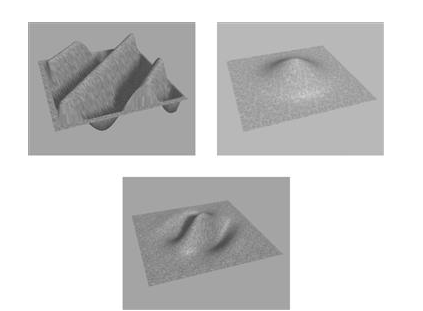
\includegraphics[width=0.5\linewidth]{gabor.png}
        \caption{Gabor detector, a sine wave multiplied by a Gaussian envelope}
    \end{figure}

\end{multicols}
\end{mdframed}



\begin{mdframed}\begin{multicols}{2}
\subsection{Pre-attentive processing and ease of search}
\begin{compactdesc}
    \item[Preattentive processing] captures certain features, entities
        ``pop out.'' Such features can be detected despite distractors.
        Misleading name, attention and perception are tightly bound.
        Anything processed faster than 10 msec. Others are $>$ 40 msec.
    \item[Features] categorized into form, color, motion, and spatial
        position:
        \begin{compactenum}
        \item Line orientation
        \item Line length, width
        \item Size
        \item Curvature
        \item Spatial grouping
        \item Blur
        \item ``Added marks''
        \item Numerosity
        \item Color, hue, intensity
        \item Motion, direction of
        \item Flicker
        \item Direction of motion
        \item Spatial position
        \item 2D position
        \item Stereoscopic depth
        \item Convex/concave from shading
        \end{compactenum}
    \item[Attention and expectation] subjects can ignore features if unexpected.
    \item[Highlight] an object by granting it a positively asymmetric
        pre-attentive cues, such as color in a black and white field.
        Subtle motion in static display.
    \item[Redundant features] can be used for more effective searches.
    \item[Not easily findable:] conjunction of features. For example: find the
        red square. Some exceptions:
        \begin{compactenum}
        \item spatial grouping on XY plane
        \item stereoscopic depth and color or movement
        \item luminance polarity (white on grey) and shape
        \item Convexity/concavity and color
        \item Motion and anything
        \end{compactenum}
\end{compactdesc}
\end{multicols}
\end{mdframed}



\begin{mdframed}\begin{multicols}{2}
    \begin{figure}[H]
        \centering
        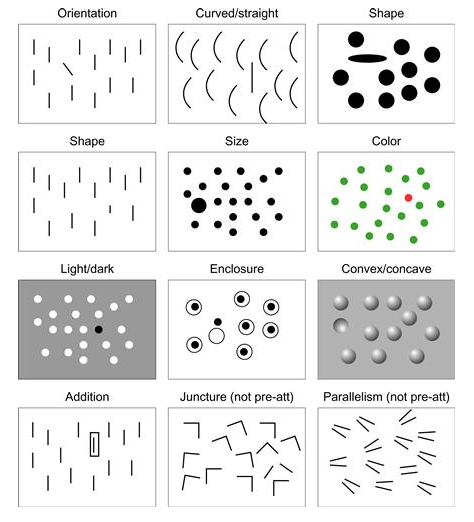
\includegraphics[width=0.25\textwidth]{preattentive.png}
        \caption{Array of preattentively processed features}
    \end{figure}


    \begin{figure}[H]
        \centering
        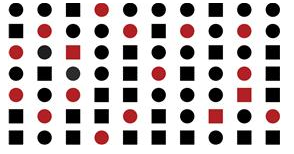
\includegraphics[width=0.3\textwidth]{find_red_square.png}
        \caption{Find the red square}
    \end{figure}

\end{multicols}
\end{mdframed}



\begin{mdframed}\begin{multicols}{2}
\subsection{Integral and separable dimensions. Glyph design.}

    \begin{figure}[H]
        \centering
        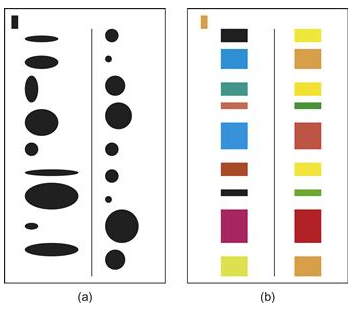
\includegraphics[width=0.5\linewidth]{speeded_classification.png}
        \caption{Speeded classification experiments. On height. In (a) the
        variable width interferes with classification. In (b) the variable
        color does not interfere}
    \end{figure}
\begin{compactdesc}
    \item[Garner's theory:] there are integral and separable dimensions.
    \item[Glyph] symbols representing quantity
    \item[Questions answered:]
        ``Will the color-scheme interfere with glyph size?''
        ``Will using both color and size make a variable clearer?''
        Will displays be perceived independently from each other?
    \item[Integral display dimensions] two attributes are perceived
        holistically and not independently
    \item[Separable dimensions] separate judgments can be made about
        each graphical dimension.
\end{compactdesc}
    \begin{figure}[H]
        \centering
        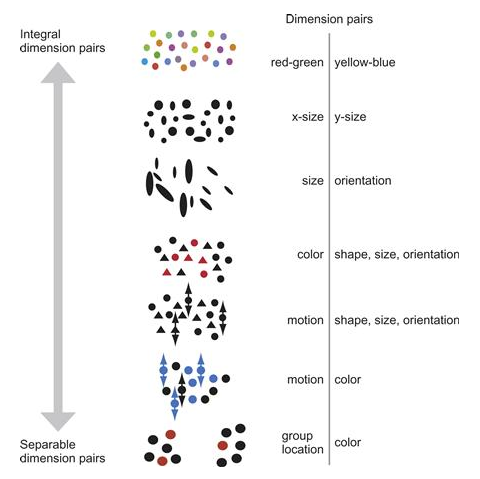
\includegraphics[width=0.5\textwidth]{integral_separable.png}
        \caption{Integral and separable dimension pairs}
    \end{figure}

\end{multicols}
\end{mdframed}



\begin{mdframed}\begin{multicols}{2}
\subsection{Representing quantity}
\begin{compactdesc}
    \item[Monotonic visual qualities] increase continuously: size,
        brightness, height. Cyclic: angle, phase of motion, hue.
    \item[Ranking] height $>$ area $>$ 3D volume $>$ grayscale.
        Area can convey greater variations.
    \item[Exact quantities] numerical annotation, bar graph, wind barb (can
        encode 30 steps, but distort wind direction).
    \item[Multidimensional discrete data]
        These are the most useful attributes in glyph design
    \begin{compactdesc}
        \item[Spatial position] 3 dimensions, XYZ
        \item[Color] 3 dimensions, color opponent theory
        \item[Shape] ?, size, orientation are basic, may be more, dimensions are
            certainly small
        \item[Surface texture] 3 dimensions, orientation size and contrast.
        \item[Motion coding] 2-3 dimensions, phase is critical, more research
            needed
        \item[Blink coding] 1 dimension, interdependent with motion
    \end{compactdesc}
        Number of resolvable steps is small. Conjunctions are not generally
        pre-attentive, unfortunately limiting us to about 32 distinct glyphs.
    \item[Stars and whiskers]
        No natural mappings to channels? Use whisker/star plots. Each variable
        is a line emanating from the center. Four whiskers is probably the
        maximum. Use parallel coordinates in case of multiple data.
    \begin{figure}[H]
        \centering
        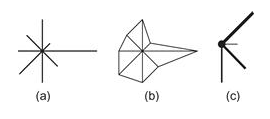
\includegraphics[width=0.2\textwidth]{whisker_star.png}
        \caption{(a) whisker plot, (b) star plot, (c) whisker with four variables and varying width}
    \end{figure}
\end{compactdesc}
\end{multicols}
\end{mdframed}


\begin{mdframed}\begin{multicols}{2}
\subsection{Searchlight metaphor and cortical magnification}
\begin{compactdesc}
    \item[Searchlight] consider the eyeball as an information-gatherer.
        Information comes in bursts, snapshot for each fixation. Nonpreattentive
        objects arrive at 40 items per second.
    \item[Useful field of view] we can quickly take information from here.
        Varies greatly, from 1 to 4 degrees of visual angle for densely
        populated targets. Can be as large as 15 degrees.
    \item[Tunnel vision] the UFOV can be extremely compressed under large
        cognitive load. Consider this when designing user interrupts.
    \item[Role of motion in attention] UFOV is larger when detecting moving
        targets. UFOV around 40 degrees.
    \item[User interrupts]
        \begin{compactenum}
        \item easily perceived, even outside of fovea
        \item can be ignored, serve as reminder
        \item non irritating
        \item can be endowed with varying levels of urgency
        \end{compactenum}
    \item[Motion as a user interrupt]
        Ship alarm flash patterns: subjects ID'd five patterns with 98\%
        reliability. Motion/blinking are reliable, but can be annoying.
        Slow motion need not be.
\end{compactdesc}
\end{multicols}
\end{mdframed}




